\title{Mapeamento de solos no nosso tempo}
\author{por Marcos Bacis Ceddia}
\maketitle
\section{Apresentação}
\begin{wrapfigure}{l}{0.15\textwidth}
 
\includegraphics[width=0.15\textwidth]{figuras/bacis}
\end{wrapfigure}
Nos últimos anos, em função do desenvolvimento e disponibilização de tecnologias digitais, a área de mapeamento de solos vem passando por um processo intenso de transformação. A transformação em curso é muito abrangente, implicando em mudanças não somente dos procedimentos técnicos de mapeamento de solos (atividades de escritório, campo e laboratório), mas também de como a informação de solos é transmitida para a sociedade (ensino e extensão). Obviamente, dada a abrangência da transformação, é natural que surjam grandes incertezas, e também oportunidades. Para que instituições e procedimentos mudem, as pessoas precisam mudar. A mudança a que me refiro não é o de negação ao passado e sim de seu completo entendimento, valorização e correta conexão com o nosso tempo e também com o futuro. Precisamos disso para dar continuidade a uma rica história de mapeamento e de conhecimento dos solos de nosso território. Por isso, o título desse texto é o ``Mapeamento de Solos no Nosso Tempo''.
\section{Contexto e objetivos}
Esse texto se baseia amplamente na palestra por mim apresentada no XXXIV Congresso Brasileiro de Ciência do Solo intitulada \emph{``Interfaces entre o Mapeamento Convencional e Digital de Solos''}, a qual ocorreu em julho de 2013 no município de Florianópolis. A palestra foi apresentada no simpósio 17 sobre Pedometria: Mitos e fatos. O tema do referido simpósio foi motivado pela percepção de que precisamos avançar na área de mapeamento de solos no Brasil. Sendo o Brasil um país de dimensões continentais e com históricos problemas de aplicação de recursos e logística para mapear sistematicamente o território, precisamos mais do que nunca, integrar pessoas e instituições, e otimizar recursos para aumentar a quantidade e melhorar a qualidade da informação de solos. É pouco provável que conseguiremos atender essas demandas nacionais se deixarmos que perdurem algumas polêmicas e mitos, as quais acabaram criando grupos que se identificam como \emph{``Mapeadores convencionais ou tradicionais e Mapeadores digitais''}
.\\
Os objetivos desse texto são:
\begin{enumerate}
\item Apresentar uma visão pessoal sobre o futuro do mapeamento de solos, abordando questões conceituais, vantagens e desvantagens, desafios e oportunidades;
\item Reapresentar o tema ``Mapeamento de solos'' de forma que possamos dar continuidade e soluções ao desafio de mapear solos no Brasil.
\end{enumerate}
\section{Para Reflexão}
Para reflexão apresento aqui uma pergunta.
\begin{center}
\textbf{Se Vasily Vasil'evich Dokuchaev e Hans Jenny estivessem vivos no século 21, e ainda estivessem trabalhando com pedologia, o que estariam pesquisando?} 
\end{center}
Não parece razoável achar que não estivessem trabalhando com as novas abordagens e tecnologias disponíveis. De fato, \cite{Jenny:1941} já havia escrito em seu livro ``Factors of Soil Formation'' (pág. 262), sua percepção das limitações de seu tempo \citep{ScullEtAl:2003}. Texto traduzido abaixo:\\
\emph{``A conversão do conhecimento fundamental relacionado à relação solo ambiente sob condições específicas de campo é impossível a menos que seja conhecida a distribuição espacial dos fatores de formação''.}\\
A distribuição espacial dos fatores de formação do solo é hoje mais acessível, como consequência de nosso tempo. No nosso tempo, temos imagens de satélite, sensores mais modernos para mapeamento de covariáveis, ferramentas matemáticas e computacionais que permitem processamento de grande quantidade de dados. Logo é de se esperar que podemos avançar ainda mais na geração de grande volume de informação de solos com maior qualidade e detalhamento.\\
Cabe aqui também uma reflexão sobre o nosso tempo. O nosso tempo é um tempo cada vez mais digital, onde tudo é rápido, eficiente, com muito apelo visual, e, portanto fascinante; mas também é um tempo que incentiva o individualismo, onde tudo é descartável e com tendência a se desconectar da realidade. O nosso tempo é um tempo que exige a sabedoria de aproveitar sua fascinação, sem, contudo nos tornarmos individualistas, sem noção dos valores do passado e das pessoas, e desconectados do mundo real.\\
O mapeamento de solos se tornará mais rápido e de melhor qualidade se tivermos a sabedoria de integrar a experiência dos pedólogos e dos dados gerados por eles, com a tecnologia disponível. Estamos falando da necessidade de uma interface, de uma continuidade. Daí a questão fundamental. Como fazer a interface?
\section{O que é um mapa, o que mapear, para que e para quem os fazemos?}
Para iniciar é pertinente apresentar em que consiste um mapa de solos, quais as questões fundamentais a serem enfrentadas no processo de mapeamento, bem como para quê fazemos mapas de solos. Sob a ótica de modelos, um mapa de solos pode ser entendido como \emph{``um modelo da distribuição espacial de classes e/ou atributos de solos em uma determinada área de interesse''}. Para gerar esse mapa, tanto no passado como hoje, de modo geral, as seguintes questões devem ser atendidas:
\begin{enumerate}
\item Atende as demandas? - Para que e para quem
\item Quanto tempo para executar?
\item Qual é o modelo de predição utilizado?
\item Qual o custo e a acurácia do mapa?
\end{enumerate}
Independente de todas as questões teóricas e dos interesses da comunidade acadêmica e científica justificamos nossos projetos e fazemos mapas para atender a demanda da sociedade por \underline{Informação de Solos}. Informação essa que deve ser utilizada no Diagnóstico, Planejamento e Tomada de decisão.\\
O mapeamento digital de solos, como também o ``convencional'', tenta responder estas questões acima apresentadas. Portanto, os pedólogos de hoje e de ontem têm a mesma responsabilidade e o que muda efetivamente são os meios tecnológicos e a capacidade de utilizar e transmitir a nossa herança de conhecimento de solos.\\
Com relação à discussão sobre o que mapear, é crescente a percepção de que o mapa de variabilidade espacial de \underline{\textbf{atributos do solo}}, diretamente relacionados aos fenômenos e demandas de interesse prático, são preferidos pelos usuários finais. Por exemplo, para um órgão governamental interessado em criar um sistema de alerta para prevenção de acidentes devido a movimentos de massa, (como aqueles que ocorrem com certa freqüência nos estados do Rio de Janeiro e Santa Catarina), mais importante que as classes de solos é conhecer os mapas de variabilidade espacial de espessura dos solos, capacidade de armazenamento de água, infiltração e condutividade hidráulica. Não se trata aqui de desvalorizar o mapa de classes de solos, onde encontramos uma unidade de mapeamento identificada com um nome taxonômico, o fato é que a linguagem e a representação espacial de uma unidade de mapeamento, nem sempre é adequada para atender a demanda de informação de solos que a sociedade necessita. Com exceção dos 
pedólogos e cientistas de solos, quem é capaz de interpretar e diferenciar as implicações práticas de unidades de
mapeamento com nomenclaturas, tais como: Argissolo Vermelho Amarelo e Latossolo Vermelho Amarelo? Mesmo os mapas de aptidão das terras baseados nessa forma de representação espacial, não fornecem subsídios adequados para estudos de causa e efeito de fenômenos, sobretudo quando se necessita informação em elevada resolução espacial.\\
Percebemos que o que é mapeado e a maneira como a informação de solos é disponibilizada para a sociedade é dependente da maneira como os mapas são feitos, assim
é interessante fazer uma breve análise de como fazíamos e fazemos mapas de solos.
\section{O Mapeamento ``Convencional ou Tradicional''}
O mapeamento de solos convencional reflete um tempo analógico. Os meios e ferramentas são analógicos, logo a equipe de pedólogo segue as seguintes etapas:
\begin{enumerate}
\item A equipe de pedólogos faz levantamento bibliográfico (mapas de solos e de covariáveis e relatórios sobre a região);
\item A exploração entre covariáveis e tipos de solos é feita de forma mecânica e visual, sendo portanto mais lenta e mais suscetível a erros de interpretação das relações;
\item O pedólogo comumente gera um mapa prévio em que a qualidade depende muito da experiência. Experiência adquirida não se transmite, no máximo, ensina-se como adquirir experiência, o que demanda tempo;
\item O pedólogo vai a campo, avalia a adequação de seu modelo mental, descreve perfis, coleta amostra, executa testes de campo e efetua correções específicas;
\item Com o modelo mental confirmado/corrigido, efetua-se a predição.
\end{enumerate}
Como dizia o professor Dr.~Doracy Pessoa Ramos: ``o pedólogo cria o que hoje é denominado de uma Função de Pedotransferência mental, a partir do qual gera o mapa de solos''.\\
Do ponto de vista de modelo, o mapeamento convencional se assenta da equação formalizada por \cite{Jenny:1941} onde o solo é função dos fatores de formação material de origem, clima, relevo, organismos e tempo (também referida em inglês como CLORPT):\\
\\
S=$f$(material de origem, clima, relevo, organismos e tempo)\\
\\
O método convencional de execução de mapeamento de solos foi o que gerou praticamente todo o acervo de informação de solos que temos no Brasil, o qual encontra-se na forma de mapas e relatórios, em sua maioria, na forma analógica.\\
De acordo com \cite{Mendonca-SantosEtAl:2007}, o mapeamento sistemático de solos do Brasil, por problemas \textbf{econômicos, institucionais e tecnológicos}, foi efetuado em escala de \underline{reconhecimento e exploratório} (escalas que variam de 1:250.000 a 1:2.500.000). Abaixo é apresentado um resumo da cronologia dos trabalhos de solos no Brasil:
\begin{itemize}
\item 1947 - Iniciou-se os mapeamentos com apoio institucional (Comissão de Solos- Ministério da Agricultura);
\item 1954 e 1955 - Primeiros Mapas de Reconhecimento (RJ e SP);
\item 1960 - Melhor treinamento de equipes (Cooperação USA). Mapas da região Norte e Central do Brasil);
\item 1971-1976 RADAMBRASIL (Amazônia Legal e todo o Brasil -- 1:1. 000.000);
\item 1974 - Desaceleração progressiva dos mapeamentos;
\item 1981 - Primeiro mapa nacional (1:5. 000.000);
\item 2001 - Mapa nacional atualizado.
\end{itemize}
Analisando a cronologia do mapeamento, bem como das informações da literatura sobre o mapeamento nacional de solos, alguns fatos são destacados, são eles: \begin{itemize}
\item Precisamos de mapas com maior detalhamento, sobretudo no interior do Brasil;
\item Os mapas geralmente não são validados no campo;
\item O processo de mapeamento é mais lento e suscetível a erros;
\item O método é menos sustentável no tempo - Como todo ser humano, o pedólogo morre. E com ele vai a experiência.
\end{itemize}
Com a desaceleração do mapeamento sistemático de solos no Brasil, reduziu-se sensivelmente a formação de pedólogos com capacitação para execução de mapas. Consequentemente, ocorreu um hiato entre a geração que executava sistematicamente os mapas e a geração de hoje. Relativamente, temos menos pedólogos com elevada experiência de campo o que contribui também para o surgimento de alguns mitos, tais como essas afirmativas:
\begin{itemize}
\item ``Os mapas convencionais não tem qualidade'';
\item ``Não tem como avaliar a acurácia do mapa''.
\end{itemize}
Na verdade quem já teve a oportunidade de utilizar e avaliar os mapas gerados concorda que os mapas têm sim qualidade adequada à sua escala de publicação. A acurácia do mapa pode ser testada, implicando na execução de campanhas de validação de campo para que se possam apresentar índices, tais como exatidão global e Índice Kappa, por exemplo. O que se pode argumentar é a não possibilidade de avaliar o modelo mental que o pedólogo usou para gerar o mapa. Em outras
palavras, o modelo, o qual não temos acesso, pode ter acertado por acaso.\\
Ainda com relação à acurácia do mapa convencional, a comum ausência de índices reflete um problema inerente a qualquer método de mapeamento, ou seja o elevado custo para efetuar campanhas de campo. Logo, é pertinente lembrar que os pedólogos brasileiros sempre enfrentaram fortes restrições orçamentárias e de logística. Esse
problema não é somente encontrado no Brasil, por exemplo, \cite{BurroughEtAl:1971} já atestava que por razões de tempo e custo, usualmente, menos de 0.001\% da área levantada é de fato observada. Abaixo estão apresentadas as principais críticas associadas ao método convencional:
\begin{itemize}
\item O modelo é implícito e totalmente dependente da experiência do pedólogo;
\item Informação incompleta a respeito dos produtos derivados do levantamento de solos;
\item Os mapas não são testados no que se refere à seu modelo de predição;
\item Sua origem atrelada na classificação taxonômica implica em uma visão de objeto. O mapa fornece uma falsa impressão de que a variação dos solos é pontual, o que de fato não reflete a realidade. O solo e seus atributos, comumente, variam no espaço e no tempo de forma contínua.
\end{itemize}
Apesar de todas as críticas e das dificuldades enfrentadas pelos pedólogos para conhecer, explicar e mapear os solos do Brasil, o fato é que existe um grande acervo de dados e mapas com qualidade. No entanto, esses mapas e dados estão dispersos e em formato analógico, e no melhor dos casos, em planilhas do tipo Excel. O conjunto de dados que temos é importante, no entanto, podemos dizer que esta muito pouco disponível para todas as instituições e pesquisadores. Guardada a devida
proporção, é como o petróleo da camada do Pré-sal, existe, mas ainda não esta disponível, até que encontremos um meio eficiente de acessa-lo. Se não organizarmos esses dados em um sistema de gerenciamento banco de dados, estaremos correndo sérios riscos de perdê-los, da mesma forma que perdemos, com o passar dos tempos, a experiência adquirida pelos pedólogos.
\section{O Mapeamento Digital}
O mapeamento digital de solos (MDS) surge  no  contexto  de  um  tempo onde dispomos de várias ferramentas digitais e também do amadurecimento de pesquisas que tentam atingir os seguintes objetivos:
\begin{enumerate}
\item Produzir mapas com acurácia declarada, com menor intensidade de trabalho de campo, tempo e custo;
\item Melhor representar a variabilidade espacial (visão de campo - modelo raster de representação);
\item Apresentar o modelo de predição de forma que seja possível sua reprodução e avaliação por outros pesquisadores.
\end{enumerate}
Por definição o MDS é ``a criação e população de sistemas de informação espacial de solos através de modelos numéricos, inferindo a variação espacial e temporal de classes e atributos de solos \underline{a partir de observações de solos e conhecimento} e variáveis ambientais correlacionadas'' \citep{McBratneyEtAl:2003}. De modo similar ao mapeamento convencional, o MDS se assenta em um modelo similar ao de \cite{Jenny:1941}, o qual é denominado SCORPAN. De acordo com \cite{McBratneyEtAl:2003}, a formulação do SCORPAN é uma descrição quantitativa empírica das relações entre o solo e outros fatores espacialmente referenciados com o objetivo de usá-los como uma função de predição espacial de solos. O termo SCORPAN é um acrônimo composto pelas primeiras letras de sete fatores interferindo no processo de predição:\\
\\
$S=f(s, c, o, r, p, a, n)$\\
\\
onde:\\
\emph{S}: Classe de solo ($S_c$) ou atributo do solo ($S_a$) a ser predito;\\
\emph{f}: é a função de predição;\\
\emph{s}: solo, outras propriedades do solo em um determinado local;\\
\emph{c}: clima, propriedades climáticas do ambiente em um determinado local;\\
\emph{o}: organismo, vegetação ou fauna ou atividade humana;\\
\emph{r}: relevo, atributos do relevo;\\
\emph{p}: material de orígem, litologia;\\
\emph{a}: tempo, o fator tempo;\\
\emph{n}: espaço, posição no espaço (coordenadas espaciais x e y).\\
O fator solo (s) é incluído porque um atributo do solo pode ser predito a partir de outros atributos ou classe, ou a classe de solo ser predita a partir conhecimento de atributos ou mesmo de classes previamente conhecidas.\\
De modo geral, durante a geração dos mapas digitais, o pedólogo segue etapas similares ao mapeamento convencional, a diferença se mostra na aplicação de ferramentas estatísticas (mineração de dados, estatística multivariada), na aplicação de algoritmos matemáticos que visam automatizar e otimizar o procedimento amostral (exemplo: hipercubo latino), na explicitação do modelo de predição e sua estimativa de erro. As etapas gerais do MDS são apresentadas abaixo:
\begin{enumerate}
\item Explorar e identificar de forma eficiente as relações entre as covariáveis preditoras e a variável as ser predita (classe ou atributo do solo);
\item Incorporar explicitamente na forma de equações ou regra de classificação, as relações entre as variáveis preditores e atributos ou classes de solos;
\item Aplicar o modelo de predição e avaliar a acurácia do modelo através de campanhas de campo (validação);
\item Geração do mapa final e relatórios.
\end{enumerate}

Um aspecto importante da etapa 3 do MDS, mais especificamente da aplicação do modelo, é que o modelo de predição é na verdade um processo automático de classificação. Esse processo automatizado de classificação acelera sensivelmente a geração de mapas, sobretudo quando se faz mapas de grandes áreas.\\
Como qualquer método, o MDS também tem desvantagens ou críticas, tais como as apresentadas abaixo:
\begin{enumerate}
\item Não disseminação de um protocolo de condução dos trabalhos de mapeamento digital.
\item Exige demasiado conhecimento de estatística e domínio de software.
\item Basicamente, a maioria dos modelos de predição gerados são predominantemente dependentes de poucas covariáveis, sobretudo derivadas do relevo e de imagens de satélite;
\item A limitação na disponibilidade de covariáveis em mesma resolução espacial implica que os algoritimos classifcadores apresentam menor capacidade de discretização de classes de solos em mapas mais detalhados;
\end{enumerate}
A ausência de um protocolo básico de procedimento de execução de MDS, nos mesmos moldes dos documentos já existentes para mapeamento convencional de solos (tais como o publicado pela EMBRAPA, 1995 - Procedimentos Normativos de Levantamentos de Solos), associado à necessidade de maior conhecimento estatístico e de software para execução de MDS, tem contribuído para a criação de um mito recorrente, que é a falsa impressão de que ``Mapas digitais são feitos sem a etapa de levantamento
de campo''.\\
Na verdade, o MDS exige a mesma atenção no trabalho de campo que um mapeamento convencional. Isso é necessário, pois o estabelecimento das relações quantitativas entre os tipos de solos e/ou atributos e as covariáveis utilizadas no modelo de predição precisam ser cuidadosamente conferidas no campo. Por exemplo, se um ponto de coleta ou perfil de solo descrito no campo for incorretamente descrito, coletado e georreferenciado, a relação entre o tipo ou atributo do solo e a posição no espaço, fornecerá uma informação equivocada dos padrões solo/paisagem. Essa informação equivocada será reproduzida pelo algoritmo de mapeamento, reproduzindo sistematicamente o erro para toda a área mapeada. Assim, o MDS acaba exigindo os mesmos cuidados do mapeamento convencional, acrescido do controle sobre todas as etapas estatísticas e de operação do algoritmo classificador.\\
A menor capacidade de discretização de mapas digitais de classe de solos em relação aos convencionais, é frequentemente observada. Uma das razões desses resultados é a ainda pouca variedade de covariáveis com mesma resolução espacial que permitam separar unidades de mapeamento. Em outras palavras, são raros os mapas de material de origem, organismos e clima, na mesma resolução que os de derivadas do relevo. Assim, é comum observar que mapas digitais apresentem melhor acurácia quando estão apresentados em escalas compatíveis com semi detalhados (ou menor  detalhamento).
\section{O que tiramos sobre os métodos de mapeamento de solos}
Quando olhamos em maior detalhe o que se fez e o que se pode fazer com os dados existentes, utilizando as alternativas modernas, nota-se que os mapas e dados de solos gerados pelo método convencional são de qualidade e não podem ser perdidos. Também fica claro que seria uma grande irresponsabilidade deixar de transformar os dados existentes em informação disponível à sociedade. O mapeamento do nosso tempo é aquele que faz a interface entre o convencional e o digital e gera e disponibiliza informação acurada de solos de forma mais rápida e com menor custo.
\section{Como se faz a interface?}
Uma maneira de se visualizar a forma pela qual a interface entre o mapeamento convencional e o digital pode ser feita é através da contextualização no modelo SCORPAN (Figura \ref{fig:esquema}). O conhecimento pode ser obtido através do uso direto dos dados de solos existentes e/ou diretamente com os pedólogos que desenvolveram atividades em uma determinada área de interesse \citep{Lagacherie:2008}.\\
\begin{figure*}[tb!]
\begin{minipage}[t]{1\linewidth}
\begin{center}
   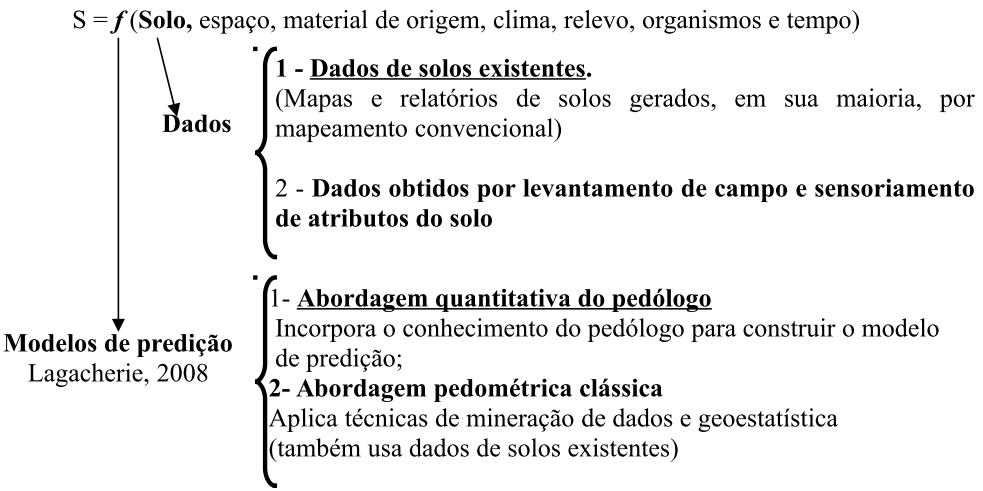
\includegraphics[width=\textwidth]{figuras/marcos-esquema}
   \caption{As possibilidades de interface entre o mapeamento convencional e o digital contextualizando no modelo SCORPAN}
   \label{fig:esquema}
 \end{center}
\end{minipage}
\end{figure*}
Quando o dado existente de solo é usado diretamente, esta interface se dá como sendo o fator solo. Nesse caso um exemplo seria a utilização de um mapa de
variabilidade espacial de um atributo do solo, considerado útil para discretização de classes ou mesmo a geração de mapa de outro atributo do solo. O mesmo dado de solo pode também gerar um modelo de predição ($f$), por exemplo, um modelo de regressão linear múltipla para predição espacial de um atributo (Água Disponível Total) a partir de outros atributos do solo (areia, argila, carbono) e de covariáveis (declividade, curvatura, índice topográfico de umidade). Nesse caso, a
mineração de dados é bastante útil para extrair ou ajudar a evidenciar padrões nestes dados e auxiliar na descoberta de conhecimento sobre solo e covariáveis. Esse conhecimento pode resultar em diversos produtos, tais como agrupamentos, hipóteses, regras, árvores de decisão, redes neurais e etc.\\
No segundo caso, o conhecimento do pedólogo é incorporado no modelo através de consulta direta, ou através da análise conjunta de mapas de solos e de covariáveis. Quando se consulta o pedólogo diretamente, o conhecimento pode ser incorporado através da construção de uma função de predição espacial ($f$), por exemplo, sistemas especialistas (implementação de regras de probabilidade condicional Bayesiana, lógica Fuzzy, e leis físicas simplificadas explicando a distribuição espacial de atributos do solo).\\
Outra forma de introdução do conhecimento de solos e covariáveis no MDS é a extração das relações solo/covariáveis diretamente no produto final de um levantamento de solos, no caso o próprio mapa. Nesse caso, por escolha ou indisponibilidade, não se consulta o pedólogo e sim o produto de seu modelo mental. O mapa, por refletir o modelo mental, é suficiente para extrair relações solo/covariáveis e construir um modelo de predição espacial. Um exemplo de extração desses padrões é a técnica da Área de Referência (AR).\\
De acordo com \cite{LagacherieEtAl:1995} muita pesquisa tem sido focada no uso inovativo de mapas de solos, tanto como uma fonte de dados para modelos de avaliação das terras ou como uma fonte adicional de informação para melhorar a eficiência de técnicas de interpolação, como a krigagem. Estes estudos tem demonstrado a
eficiência de mapas detalhados de solos (\textgreater{}1:25.000). No entanto, mapas detalhados não estão disponíveis em grande parte do território dos países, sobretudo no Brasil. Pensando em superar essa deficiência, \cite{Favrot:1981} propôs o método da Área de Referencia (AR). O objetivo desse método é caracterizar a cobertura de solos de regiões topograficamente e geologicamente identificáveis, denominadas ``pequenas regiões naturais''. O primeiro passo desse método consiste em efetuar o mapeamento detalhado de uma pequena, mas representativa área, de uma pequena região natural, a qual é denominada A.R.. Nesta A.R. caracterizam- se as principais classes de solos de toda a região e se estabelecem as regras de mapeamento. Esta primeira etapa facilita e acelera a etapa seguinte, a qual consiste na condução de novos trabalhos de mapeamento em áreas circunvizinhas. Na condução dos novos trabalhos de mapeamento, são levantados novos pontos de observação onde se esperam encontrar as mesmas classes de solos 
identificadas e mapeadas na A.R. Assim, também se espera poder fazer o delineamento dos limites de unidades de mapeamento a partir das regras de mapeamento preestabelecidas na A.R.\\
Quando se desenvolve mapeamento tendo como base o método da A.R., o que esta sendo testado é a hipótese de que é possível delimitar áreas (denominadas ``pequenas áreas naturais'') que englobem um número finito de classes de solos, as quais são recorrentes em associação umas com as outros na paisagem e formando um padrão repetitivo e identificável. Desta forma, uma A.R. propositalmente escolhida seria suficiente para identificar todas as classes de solos de uma área maior e também determinar suas relações espaciais. Segundo \cite{LagacherieEtAl:1995} a hipótese assumida no método da A.R. ainda precisa ser experimentalmente confirmado, embora já existam estudos, sobretudo na França, demonstrando que o método de A.R. é satisfatório. Ainda segundo \cite{LagacherieEtAl:1995}, os resultados obtidos na França
demonstram que os trabalhos efetuados utilizando A.R. tem reduzido a necessidade de trabalhos de campo, e que em geral menos de 10\% das unidades de solos encontradas nas novas áreas são diferentes daquelas estabelecidas nas A.R. Por outro lado, o mesmo autor observa que os ganhos de eficiência obtidos quando se aplicou a técnica de A.R. é obtida quando a equipe que faz os mapeamentos de outras áreas é a mesma que participou do trabalho da A.R. Assim, a desvantagem do método da A.R. é que a experiência obtida durante o mapeamento da área de referencia parece não ser ainda adequadamente explicitadas nos relatórios e mapas publicados, limitando sua transferência a outros pedólogos. Para contornar a limitação do método, \cite{LagacherieEtAl:1995} e outros pesquisadores, tem apresentado procedimentos computadorizados de levantamento de solos onde se procura reproduzir o raciocínio que um pedólogo experiente segue durante um levantamento realizado após uma pesquisa em uma área de referência.\\
De acordo com \cite{WalterEtAl:2007}, dois tipos de regras de conhecimentos de especialistas tem sido derivadas de mapas de solos, as quais são denominadas ``regras solo paisagem'' e `` regras de padrão de solos''. No primeiro caso (solo paisagem) utilizam-se como preditores os fatores do modelo SCORPAN, tais como derivadas do MDE e de sensores remotos para predizer classes de solos em lugares não visitados. Para a predição tem sido utilizados algorítimos como arvores de decisão \citep{Lagacherie:1992, LagacherieEtAl:1997, BuiEtAl:1999}, as quais fornecem um conjunto de regras de probabilidades de predição de unidades de mapeamento de solos.  No segundo caso (regras de padrões de solos), regras de padrões de distribuições de solos são capturadas nas áreas de referencia para inferência em uma área de interesse. Neste caso, utiliza-se como exemplo ilustrativo a ocorrência de três tipos de unidades de mapeamento, aqui denominadas A, B e C. Se o pedólogo observa
que na área de referencia, sistematicamente, a unidade de mapeamento C ocorre entra as unidades de mapeamento A e B, então cria-se uma regra de padrão de distribuição onde essa variação sistemática é transformada em regra de mapeamento. Assim, por exemplo, poder-se-ia determinar uma distância na qual, dado a presença da unidade C, encontrar-se-ia as probabilidades de ocorrência das unidades B e A. \cite{LagacherieEtAl:1995}, utilizou essa técnica no Valley of Herault no sul da França e considerou a técnica promissora para regiões onde padrões de distribuição de solos são identificáveis e recorrentes.\\
No Brasil a técnica de AR é ainda relativamente pouco aplicada. A técnica foi aplicada por \cite{TenCatenEtAl:2011} para mapear classes de solos no município de São Pedro do Sul-RS. Os autores concluíram que o MDS a partir de uma AR pode ser utilizado como alternativa ao mapeamento convencional para dimensões mais extensas da paisagem. A seleção de áreas de referência representativas da paisagem a ser mapeada é uma fase crucial para a adequada extrapolação das relações solo-paisagem, além da seleção de variáveis ambientais, as quais tenham forte relação com a pedogênese dos solos a serem mapeados.\\
Outro trabalho que utilizou a técnica de AR no Brasil foi o desenvolvido por \cite{Villela:2013}. O autor aplicou a técnica para mapear classes de solos sob floresta amazônica no município de Coari - AM. A partir de uma área de 7.900 hectares, a qual foi mapeada de forma convencional em escala detalhada (1:10.000), o autor desenvolveu funções discriminantes para mapear classes de solos de uma região no entorno com dimensões de 50.000 hectares, em escala 1:25.000, e de 116.000 hectares em escala 1:50.000. Os resultados de \cite{Villela:2013} e de \cite{TenCatenEtAl:2011} indicam que a técnica de AR é promissora. Os autores destacam a necessidade de desenvolver maiores estudos de validação e destacam a necessidade de avaliar a dimensão espacial da validade das extrapolações feitas a partir de uma área de referência.
\section{Demandas e desafios da interface}
Quando  avaliamos  as  possibilidades  de  interface,  dois  aspectos básicos se destacam, o primeiro refere-se à necessidade de um Sistemas de Gerenciamento de Banco de Dados de solos (SGBDsolos), e o segundo é a necessidade de aproximação entre diferentes gerações de pedólogos. A criação de um SGBDsolos é uma grande demanda, pois alem de permitir a organização e preservação do acervo de dados, permitirá o trabalho mais eficiente de mineração de dados por diversas instituições. No entanto, o assunto banco de dados é bastante complexo, pois envolve questões técnicas (modelagem do banco, software e hardware), jurídicas, disponibilidade e política de dados. No Brasil, apesar da lei de acesso a informação (Lei N° 12.527 de 18/11/2011), de modo geral, não existe a cultura de acesso à informação, inclusive para dados de solos. Na verdade, ate hoje não temos um SGBDsolos e são raros os arquivos de dados e mapas de solos que podem ser acessados. Os poucos exemplos de endereço na Internet onde é possível obter dados 
e mapas de solos, são:
\begin{enumerate}
\item \href{http://www.esalq.usp.br/gerd}{Esalq} - \underline{Fonte de dados}: RADAMBRASIL. 5.479 perfis de solo; 10.950 horizontes e 57 colunas com variáveis independentes. \underline{Formato}: .xls e .mdb;
\item \href{ftp://geoftp.ibge.gov.br/mapeamento_sistematico/banco_dados_georeferenciado_recursos_naturais/latlong/}{IBGE - latlong} ou \href{ftp://geoftp.ibge.gov.br/mapeamento_sistematico/banco_dados_georeferenciado_recursos_naturais/albers/}{IBGE - albers} - \underline{Fonte}: RADAMBRASIL (incorporado ao IBGE); \underline{Formato}: .pdf, shapefile; \underline{Tipo de dados}: mapas de solos, geomorfologia, geologia e vegetação.
\end{enumerate}
Os únicos dados e mapas parcialmente disponíveis são aqueles gerados pelo projeto RADAMBRASIL.\\
Com relação à aproximação entre diferentes gerações de pedólogos, é possível que exista em algumas instituições e em momentos específicos, no entanto, ainda é muito pouco expressiva diante da grande importância. O diálogo mais frequente e sistematizado permitirá a transmissão do conhecimento e definição de estratégias de mapeamento sistemático do Brasil.\\
Quanto mais nos aprofundamos na pesquisa em MDS notamos o quão vasto é a área, o que causa uma certa sensação de impotência diante de tantas áreas importantes para serem estudadas. Destaco aqui \underline{algumas} áreas que, além do ensino formal de solos, precisam ser utilizadas para aperfeiçoamento do MDS, são elas:
\begin{itemize}
\item Treinamento em modelagem matemática;
\item Desenvolvimento de software e bancos de dados;
\item Desenvolvimento e avaliação de sensores;
\end{itemize}
Cada uma dessas áreas possui várias subdivisões e por si demandam uma vida científica, logo dificilmente uma única pessoa domina eficientemente todas as áreas de conhecimento envolvidas no MDS. Assim, parece mais razoável investir no desenvolvimento de grupos interdisciplinares. ``\underline{Não é fácil achar um Michelangelo}''.
\section{Considerações finais}
O MDS é uma realidade no Brasil e representa a melhor alternativa para atender as demandas crescentes da sociedade por informações de solos. No entanto, ainda há um caminho longo a ser percorrido para que tenhamos um processo de mapeamento sistemático do território brasileiro através do MDS. Ainda precisamos criar protocolos mínimos para o MDS, formar mais profissionais na área, produzir materiais didáticos, fazer mais reuniões cientificas com diferentes gerações de pedólogos e, sobretudo, nos atirarmos na execução de mapas de solos no território Brasileiro. A prática constante nos permitira apresentar uma alternativa sólida de mapeamento para o Brasil.\\
O MDS é por natureza multidisciplinar, portanto, o seu desenvolvimento passa pela solidificação de trabalhos através de parcerias. Trabalhos em parcerias podem acelerar a geração de resultados práticos, no entanto, são mais complexos de serem gerenciados e exigem um grau de amadurecimento de pessoas e instituições bastante elevado. Um fato inquestionável, que denota o quanto ainda temos que avançar em termos de parceria nacional, é a não existência de um sistema de gerenciamento de banco de dados de solos do Brasil. Destaco aqui algumas características que considero essenciais para o sucesso das parcerias em MDS:
\begin{itemize}
\item Ter humildade para perceber a necessidade do trabalho em grupo;
\item Trocar o conhecimento para torná-lo disponível e aplicado;
\item Ter a visão de todo o processo de mapeamento digital de forma que não nos paralisemos nas inúmeras etapas entre o planejamento do mapeamento e a entrega do produto final;
\item Saber passar ao usuário como a informação de solo lhe pode ser útil.
\end{itemize}
Desde 2011 o Brasil possui uma Rede Brasileira de Mapeamento Digital em alta Resolução, congregando pesquisadores de vários estados e instituições. O fortalecimento dessa rede é o que temos de mais próximo de um trabalho em parceria em MDS.
\begin{footnotesize}
\begin{thebibliography}{99}
\bibitem[Bui et~al. (1999) Bui, Loughhead \& Corner]{BuiEtAl:1999}
E.N. Bui, A. Loughhead \& R. Corner (1999)
\newblock Extracting soil-landscape rules from previous soil surveys.
\newblock {\em Soil Research} 37: 495-508.
\bibitem[Burrough et~al. (1971) Burrough, Beckett, Jarvis]{BurroughEtAl:1971}
P.A. Burrough, P.H.T. Beckett \& M.G. Jarvis (1971)
\newblock The relation between cost and utility in soil survey (I--III).
\newblock {\em  Journal of Soil Science} 22: 359-394.
\bibitem[Favrot (1981) Favrot]{Favrot:1981}
J.C. Favrot (1981)
\newblock Pour une approche raisonnée du drainage agricole en France: La méthode des secteurs de référence.
\newblock {\em C.R. Académie d'Agriculture de France} 716-723.
\bibitem[Jenny (1941) Jenny]{Jenny:1941}
H. Jenny (1941)
\newblock Factors of soil formation - a system of quantitative pedology.
\newblock Dover Publications, New York. 281p.
\bibitem[Lagacherie (1992) Lagacherie]{Lagacherie:1992}
P. Lagacherie (1992)
\newblock Formalisation des lois de distribution des sols pour automatiser la cartographie pédologique à partir d'un secteur pris comme référence.
\newblock {\em Thesis (PhD in Soil Science)} 175p.
\bibitem[Lagacherie et~al. (1995) Lagacherie, Legros \& Burfough]{LagacherieEtAl:1995}
P. Lagacherie, J. P. Legros \& P. Burfough (1995)
\newblock A soil survey procedure using the knowledge of soil pattern established on a previously mapped reference area.
\newblock {\em Geoderma} 65: 283-301.
\bibitem[Lagacherie \& Holmes (1997) Lagacherie \& Holmes]{LagacherieEtAl:1997}
P. Lagacherie \& S. Holmes (1997)
\newblock Addressing geographical data errors in a classification tree for soil unit prediction.
\newblock {\em International Journal of Geographical Information Science} 11: 183-198.
\bibitem[Lagacherie \& McBratney (2007) Lagacherie \& McBratney]{LagacherieEtal:2007}
P. Lagacherie, A.B. McBratney (2007)
\newblock Spatial soil information systems and spatial soil inference systems: perspectives for Digital Soil Mapping.
\newblock {\em Digital Soil Mapping, an introductory perspective. Developments in soil science} 31:3-24.
\bibitem[Lagacherie (2008) Lagacherie]{Lagacherie:2008}
P. Lagacherie (2008)
\newblock Digital Soil Mapping: State of the Art.
\newblock {\em Digital Soil Mapping with Limited Data}, pp.3-14.
\bibitem[McBratney et~al. (2003) McBratney, Mendonça-Santos, Minansny]{McBratneyEtAl:2003}
A.B. McBratney, M.L. Mendonça-Santos, B. Minansny (2003)
\newblock On Digital Soil Mapping.
\newblock {\em Geoderma} 117:3-52.
\bibitem[Mendonça-Santos \& Santos (2007) Mendonça-Santos \& Santos]{Mendonca-SantosEtAl:2007}
M.L. Mendonça-Santos, H.G. Santos (2007)
\newblock The state of the art of Brazilian soil mapping and prospects for digital soil mapping.
\newblock {\em Developments in Soil Science} 31:39-55.
\bibitem[Scull et~al. (2003) Scull, Franklin, Chadwick, Mcarthur]{ScullEtAl:2003}
P. Scull, J. Franklin, O.A. Chadwick, D. Mcarthur (2003)
\newblock Predictive soil mapping: a review.
\newblock {\em Progress in physical geography} 27:171-197.
\bibitem[Ten Caten et~al. (2011) Ten Caten, Dalmolin, Pedron, Mendonça-Santos]{TenCatenEtAl:2011}
A. Ten Caten, R.S.D. Dalmolin, F.A. Pedron, M.L. Mendonça-Santos (2011)
\newblock Extrapolação das relações solo-paisagem a partir de uma área de referência.
\newblock {\em Ciência Rural} 41: 812-816.
\bibitem[Villela (2013) Villela]{Villela:2013}
A.L.O. Villela (2013)
\newblock Mapeamento Digital de Solos da Formação Solimões - Urucu, AM.
\newblock {\em Thesis (PhD in Agronomy-Soil Science)} 110p.
\bibitem[Walter et~al. (2007) Walter, Lagacherie, Follain]{WalterEtAl:2007}
C. Walter, P. Lagacherie, S. Follain (2007).
\newblock Integrating pedological knowledge into Digital Soil Mapping
\newblock {\em Digital Soil Mapping, an introductory perspective. Developments in soil science} 31:281-300.
\end{thebibliography}
\end{footnotesize}
\address{Marcos Bacis Ceddia\\
  Universidade Federal Rural do Rio de Janeiro\\
  \url{www.aguaesolos.net}\\
  \email{marcosceddia@gmail.com}}